\section{实验:用温度计测量温度}\label{sec:2-4}

温度的测量很重要,但很可能你对温度的估计还是不够准确的。
比如,今天的气温是多少?你每天洗脸用的水的温度是多少?你能说出它们的大约数值吗?
现在我们用温度计来测量一些温度,检查我们估计温度的能力。

先观察一下将要使用的温度计,看看它能够测量的温度范围和每个刻度(每一小格)的温度值,
再回忆一下使用温度计时应该注意的问题。

然后倒一杯开水,用温度计测出它的温度。

让开水冷却到你可以饮用但觉得很烫的程度,估计这时水的温度,再用温度计实际测量。

继续让水冷却,
到你可以饮用而且觉得不烫的程度,
到你的手可以伸进去但觉得很热的程度,
到你的手伸进去觉得不冷不热的程度,
每次都事先估计水的温度,然后用温度计实际测量。

自己设计一个表格,把你每次的估计值和实测数据都填入表中。
比比看,你对温度的估计能力怎样?


\lianxi

(1) 能不能直接用体温计测量开水的温度?为什么?

(2) 利用双金属片可以制成金属温度计(图 \ref{fig:2-11})。
双金属片卷成螺线形,一端固定,另一端用一金属丝绕过转轴拉在弹簧上。
转轴上装有一个指针。从指针的示数可以读出气温。说明这种温度计的原理。
假如跟图中所示的相反,双金属片的内层是铁,外层是铜,温度升高时,指针将向哪边偏转?

\begin{figure}[htbp]
    \centering
    \begin{minipage}{8cm}
    \centering
    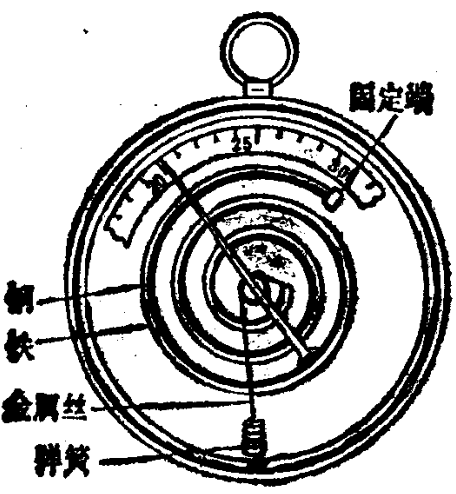
\includegraphics[width=6cm]{../pic/czwl2-ch2-11}
    \caption{}\label{fig:2-11}
    \end{minipage}
    \qquad
    \begin{minipage}{6cm}
    \centering
    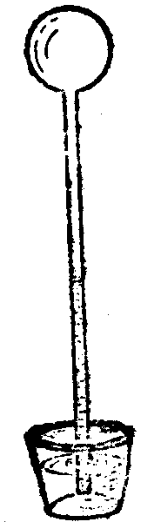
\includegraphics[width=2cm]{../pic/czwl2-ch2-12}
    \caption{}\label{fig:2-12}
    \end{minipage}
\end{figure}

\section*{小实验}

世界上第一个温度计,是伽利略根据气体的热胀冷缩的性质制成的。
它的工作原理如图 \ref{fig:2-12} 所示。
先给球形容器加热,使里面的空气跑出一部分。
停止加热,带色的液体就顺着玻璃管升上去。(为什么?)
这样就做成了一个测量气温的温度计。

想一想,伽利略是根据什么来判断气温高低的?

用这种方法测量气温,要受大气压变化的影响。
想一想,如果气温没有改变而大气压增大或者减小了,观察者将误认为气温发生了什么变化?

你想实验一下伽利略温度计的效果吗?这并不困难。
找一个空的玻璃瓶子,在它的盖子上扎一个小孔。
再找一段透明的管子(例如,拔去头的用完的圆珠笔心),把它的一端插进小孔里。
然后,设法封住瓶盖的缝隙,不让它漏气。
这样,你的伽利略温度计就做成了。

